%# -*- coding: utf-8-unix -*-
%%==================================================

\chapter{算法合集}
\label{chap10}

\begin{itemize}[noitemsep,topsep=0pt,parsep=0pt,partopsep=0pt]
	\item 这部分将关键的算法都陈列在这里了,比较有概率考到,是QQ群我的师兄分享给我的要背(或者理解能默写出来)的程序。
	\item 有一部分使用了书上的代码,比如 EQ 到时候替换为相应的C/C++代码即可
\end{itemize}

\section{背诵的集合图片}
\begin{figure}[H]
	\centering  % 环境中的内容居中排版
	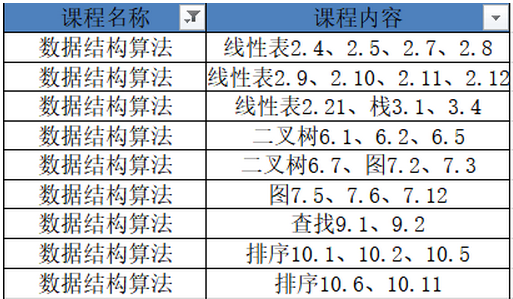
\includegraphics[scale=0.8]{example/chapter10/need.png}
\end{figure}

\section{算法实现}

\subsection{2.4}
\begin{lstlisting}[basicstyle=\small\ttfamily, caption={}, numbers=none]
算法思路:
顺序表在第i个元素之前插入一个元素时,需要移动第n个到第i个元素
\end{lstlisting}
\begin{lstlisting}[basicstyle=\small\ttfamily, caption={}, numbers=none]
Status ListInsert_Sq(SqList &L, int i, int e) {
	if (i < 1 || i>L.length + 1) return ERROR;
	if (L.length >= L.listsize) {
		newbase = (int *)realloc(L.elem, (L.listsize + LISTINCREMENT) * sizeof(int));
		if (!newbase) exit(OVErFLOW);
		L.elem = newbase;
		L.listsize += LISTINCREMENT;
	}
	q = &(L.elem[i - 1]);  // 第 i 个位置,因为从0开始的长度
	for (p = &(L.elem[L.length - 1]); p >= q; --p) { // p 指向最后一个元素,然后移动到后一个空元素
		*(p + 1) = *p;
	}
	*q = e;
	++L.length;
	return OK;
}
\end{lstlisting}

\subsection{2.5}
\begin{lstlisting}[basicstyle=\small\ttfamily, caption={}, numbers=none]
算法思路:
顺序表删除第i个元素,将第i+1至第n个元素一次向前移动一个位置
\end{lstlisting}
\begin{lstlisting}[basicstyle=\small\ttfamily, caption={}, numbers=none]
Status ListDelete_Sq(SqList &L, int i, int &e) {
	if (i < 1 || i>L.length + 1) return ERROR;
	q = &(L.elem[i - 1]);  // 第 i 个位置,因为从0开始的长度
	e = *q;
	p = L.elem + L.length - 1;
	for (q++; q <= p; ++q) { //
		*(q - 1) = *q;
	}
	--L.length;
	return OK;
}

\end{lstlisting}

\subsection{2.7}
\begin{lstlisting}[basicstyle=\small\ttfamily, caption={}, numbers=none]
算法思路:
合并两个顺序表,合并的两个顺序表也是有序的
\end{lstlisting}
\begin{lstlisting}[basicstyle=\small\ttfamily, caption={}, numbers=none]
void MergeList_Sq(SqList La, Sqlist Lb, SqList &Lc) {
	pa = La.elem; pb = Lb.elem;
	Lc.listsize = Lc.length = La.length + Lb.length;
	pc = Lc.elem = (int *)malloc(Lc.listsize * sizeof(int));
	if (!Lc.elem) exit(OVERFLOW);
	pa_last = La.elem + La.length - 1;
	pb_last = Lb.elem + Lb.length - 1;
	while (pb <= pa_last && pb <= pb_last) {
		if (*pa <= *pb) *pc++ = *pa++;
		else *pc++ = *pb++;
	}
	while (pa <= pa_last) *pc++ = *pa++;//插入a剩余元素
	while (pb <= pb_last) *pc++ = *pb++;//插入b剩余元素
}
\end{lstlisting}

\subsection{2.8}
\begin{lstlisting}[basicstyle=\small\ttfamily, caption={}, numbers=none]
算法思路:
链表得到元素
\end{lstlisting}
\begin{lstlisting}[basicstyle=\small\ttfamily, caption={}, numbers=none]
Status GetElem_L(LinkList L, int i, int & e) {
	p = L->next; j = 1;
	while (p && j<i)
	{
		p = p->next;
		++j;
	}
	if (!p || j > i)return ERROR;
	e = p->data;
	return OK;
}
\end{lstlisting}


\subsection{2.9}
\begin{lstlisting}[basicstyle=\small\ttfamily, caption={}, numbers=none]
算法思路:
链表插入元素
\end{lstlisting}
\begin{lstlisting}[basicstyle=\small\ttfamily, caption={}, numbers=none]
Status ListInsert_L(LinkList &L, int i, int e) {
	p = L;
	j = 0;
	while (p && j < i - 1) {
		p = p->next;
		++j;
	}
	if (!p || j < i - 1) return ERROR;
	s = (LinkList)malloc(sizeof(LNode));
	s->data = e;
	s->next = p->next;
	p->next = s;
	return OK;
}
\end{lstlisting}

\subsection{2.10}
\begin{lstlisting}[basicstyle=\small\ttfamily, caption={}, numbers=none]
算法思路:
链表删除元素
\end{lstlisting}
\begin{lstlisting}[basicstyle=\small\ttfamily, caption={}, numbers=none]
Status ListDelete_L(LinkList &L, int i, int &e) {
	p = L; j = 0;
	while (p->next && j < i - 1) {
		p = p->next; ++j;
	}
	if (!(p->next) || j > i - 1)
		return ERROR;
	q = p->next; p->next = q->next;
	e = q->data;
	free(q);
	return OK;
}
\end{lstlisting}

\subsection{2.11}
\begin{lstlisting}[basicstyle=\small\ttfamily, caption={}, numbers=none]
算法思路:
合并两个有序链表
\end{lstlisting}
\begin{lstlisting}[basicstyle=\small\ttfamily, caption={}, numbers=none]
void MergeList_L(LinkList &La, LinkList &Lb, LinkList &Lc) {
	pa = La->next; pb = Lb->next;
	Lc = pc = La;
	while (pa && pb) {
		if (pa->data <= pb->data) {
			pc->next = pa; pc = pa; pa = pa->next;
		}
		else {
			pc->next = pb; pc = pb; pb = pb->next;
		}
	}
	pc->next = pa ? pa : pb;
	free(Lb);
}
\end{lstlisting}


\subsection{2.12}
\begin{lstlisting}[basicstyle=\small\ttfamily, caption={}, numbers=none]
算法思路:
建立带头节点的单链线性表
\end{lstlisting}
\begin{lstlisting}[basicstyle=\small\ttfamily, caption={}, numbers=none]
void CreateList_L(LinkList &L, int n) {
	L = (LinkList)malloc(sizeof(LNode));
	L->next = NULL;
	for (int i = n; i > 0; --i) {
		p = (LinkList)malloc(sizeof(LNode));
		scanf(&p->data);
		p->next = L->next; L->next = p;
	}
}
\end{lstlisting}


\subsection{3.1}
\begin{lstlisting}[basicstyle=\small\ttfamily, caption={}, numbers=none]
算法思路:
利用栈实现非负十进制转为8进制
\end{lstlisting}
\begin{lstlisting}[basicstyle=\small\ttfamily, caption={}, numbers=none]
void conversion() {
	InitStack(S);
	scanf("%d", &N);
	while (N) {
		Push(S, N % 8);
		N = N / 8;
	}
	while (!StackEmpty(S)) {
		Pop(S, e);
		printf("%d", e);
	}
}
\end{lstlisting}


\subsection{3.4}
\begin{lstlisting}[basicstyle=\small\ttfamily, caption={}, numbers=none]
算法思路:
表达式求值
\end{lstlisting}
\begin{lstlisting}[basicstyle=\small\ttfamily, caption={}, numbers=none]
Status EvaluateExpression() {
	InitStack(OPTR); Push(OPRT, '#');//寄存运算符
	InitStack(OPND); c = getchar(); //OPND 寄存操作数或运算结果
	while (c != '#' || GetTop(OPTR) != '#') {
		if (!In(c, OP)) {
			Push(OPND, c);
			c = getchar();// 不是运算符,进栈
		}
		else {
			switch (Precede(GetTop(OPTR), c)) {
			case '<'://栈顶元素优先级低
					Push(OPTR, c); c = getchar();
					break;
			case '=':
				Pop(OPTR, x);
				c = getchar();
				break;
			case '>'://栈顶元素优先级低
				Pop(OPTR, theta);
				Pop(OPND, b);
				Pop(OPND, a);
				Push(OPND, Operate(a, theta, b));
				break;
			}
		}
	}
	return GetTop(OPND);
}
\end{lstlisting}

\subsection{6.1}
\begin{lstlisting}[basicstyle=\small\ttfamily, caption={}, numbers=none]
算法思路:
递归先序遍历
\end{lstlisting}
\begin{lstlisting}[basicstyle=\small\ttfamily, caption={}, numbers=none]
Status PreOrderTraverse(BiTree T, Status(*visit) (int e)) {
	if (T) {
		if (visit(T->data))
			if (PreOrderTraverse(T->lchild, visit))
				if (PreOrderTraverse(T->rchild, visit)) return OK;
		return ERROR;
	}
	else return OK;	
}
\end{lstlisting}


\subsection{6.2}
\begin{lstlisting}[basicstyle=\small\ttfamily, caption={}, numbers=none]
算法思路:
中序非递归算法
\end{lstlisting}
\begin{lstlisting}[basicstyle=\small\ttfamily, caption={}, numbers=none]
Status InOrderTraverse(BiTree T, Status(*Visit)(int e)) {
	InitStack(S);
	Push(S, T);//根指针进栈
	while (!StackEmpty(S)) {
		while (GetTop(S, &p) && p) Push(S, p->lchild); //向左走到尽头
		Pop(S, p); // 空指针退栈
		if (!StackEmpty(S)) {
			Pop(S, p);
			if (!Visit(p->data))
				return ERROR;
			Push(S, p->rchild);// 访问节点向右一步
		}
	}
	return OK;
}
\end{lstlisting}

\subsection{6.5}
\begin{lstlisting}[basicstyle=\small\ttfamily, caption={}, numbers=none]
算法思路:
中序线索化二叉树的遍历
\end{lstlisting}
\begin{figure}[H]
	\centering  % 环境中的内容居中排版
	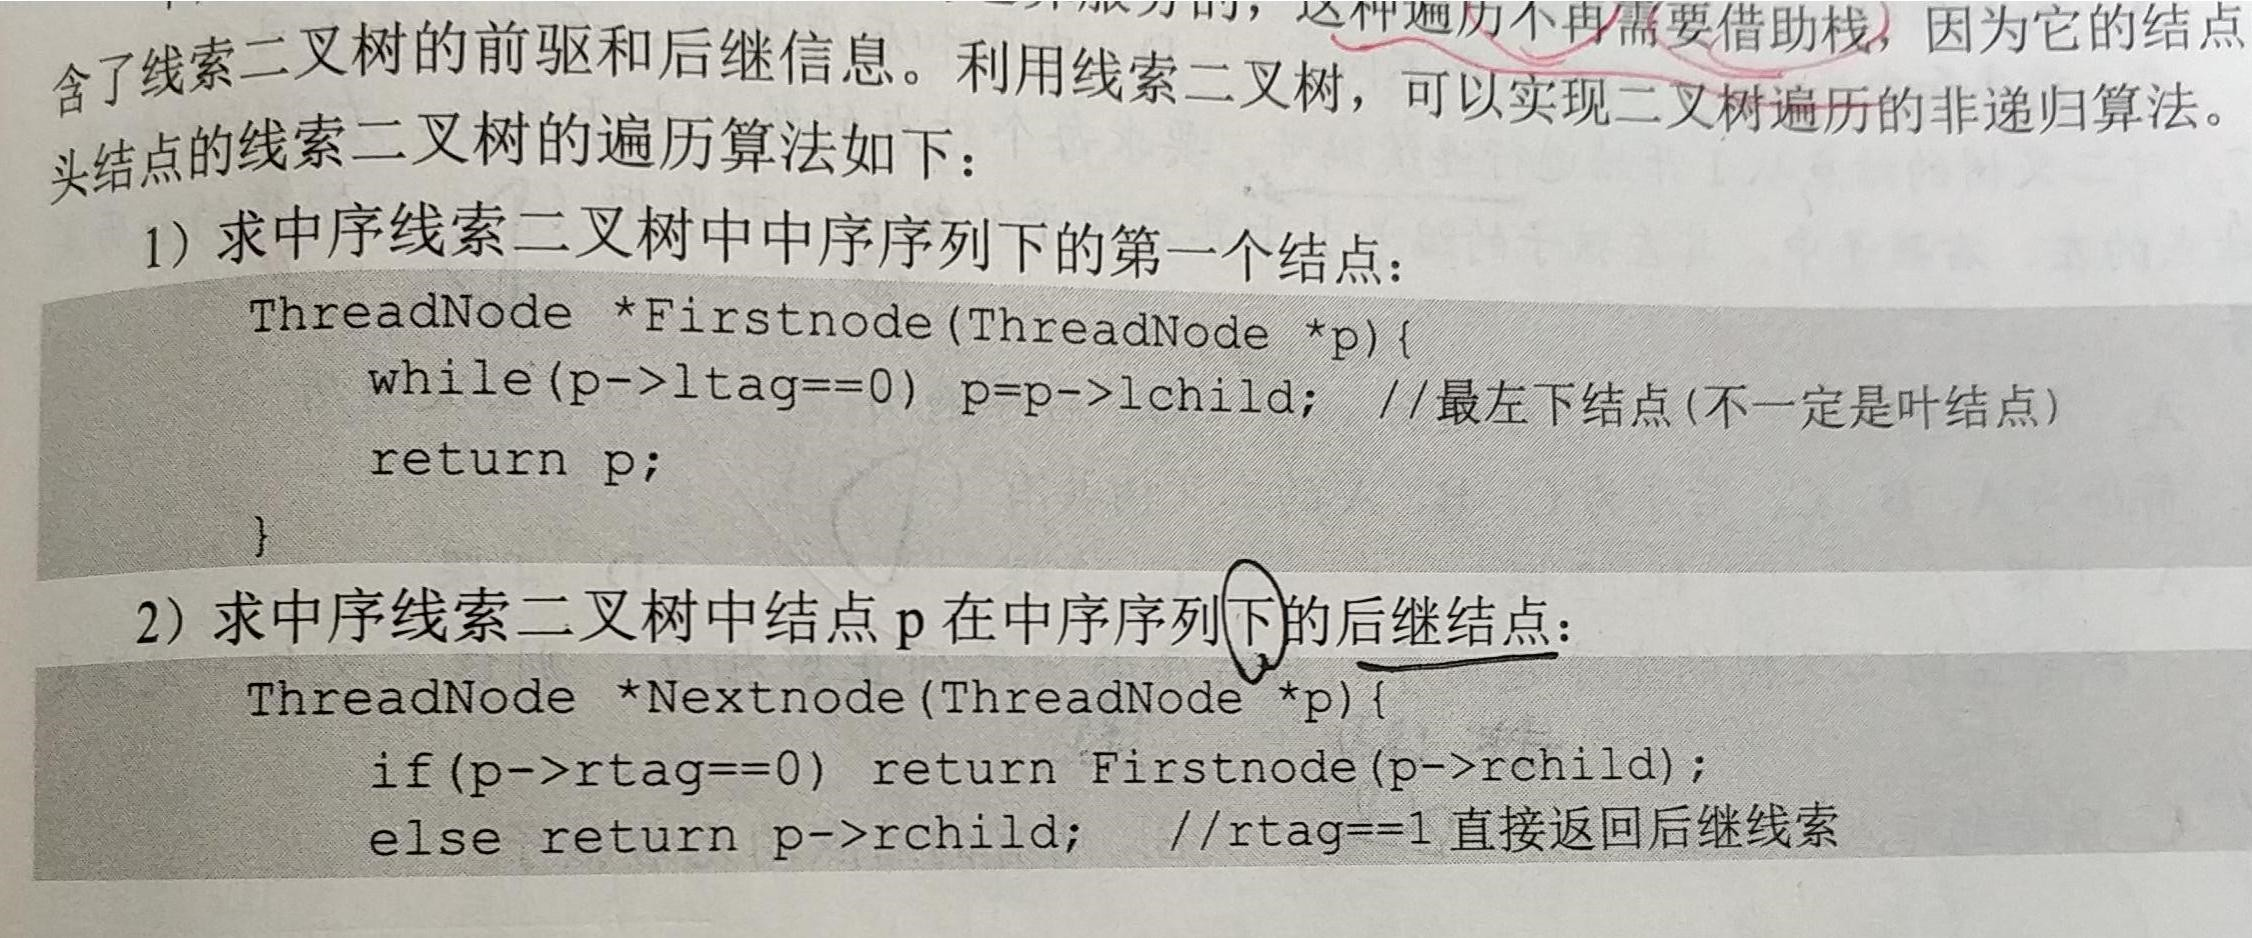
\includegraphics[scale=0.3]{example/chapter10/Img_181217111812632-1.jpg}
\end{figure}

\subsection{6.7}
\begin{lstlisting}[basicstyle=\small\ttfamily, caption={}, numbers=none]
算法思路:
中序线索化  不带头结点
\end{lstlisting}
\begin{figure}[H]
	\centering  % 环境中的内容居中排版
	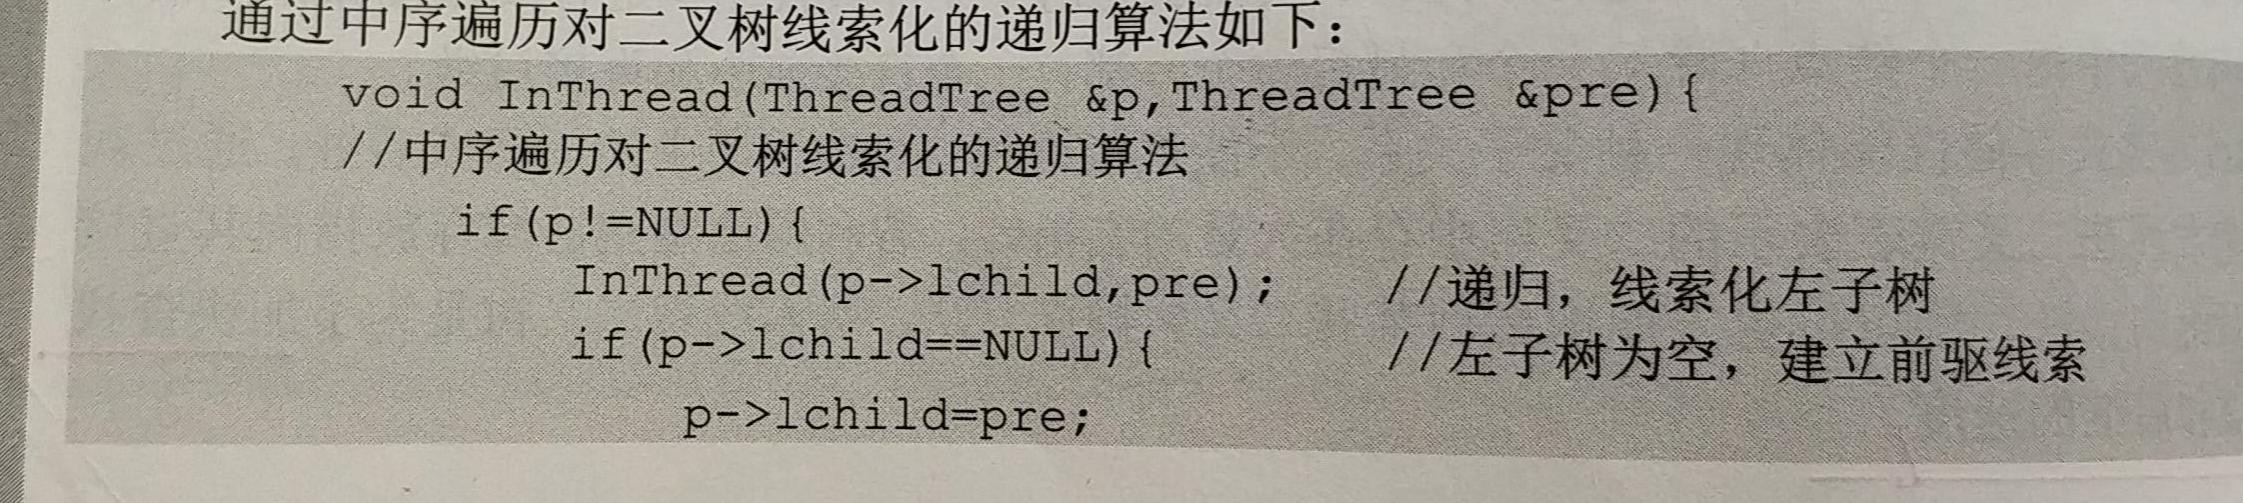
\includegraphics[scale=0.3]{example/chapter10/Img_181217112900037-1.jpg}
\end{figure}
\begin{figure}[H]
	\centering  % 环境中的内容居中排版
	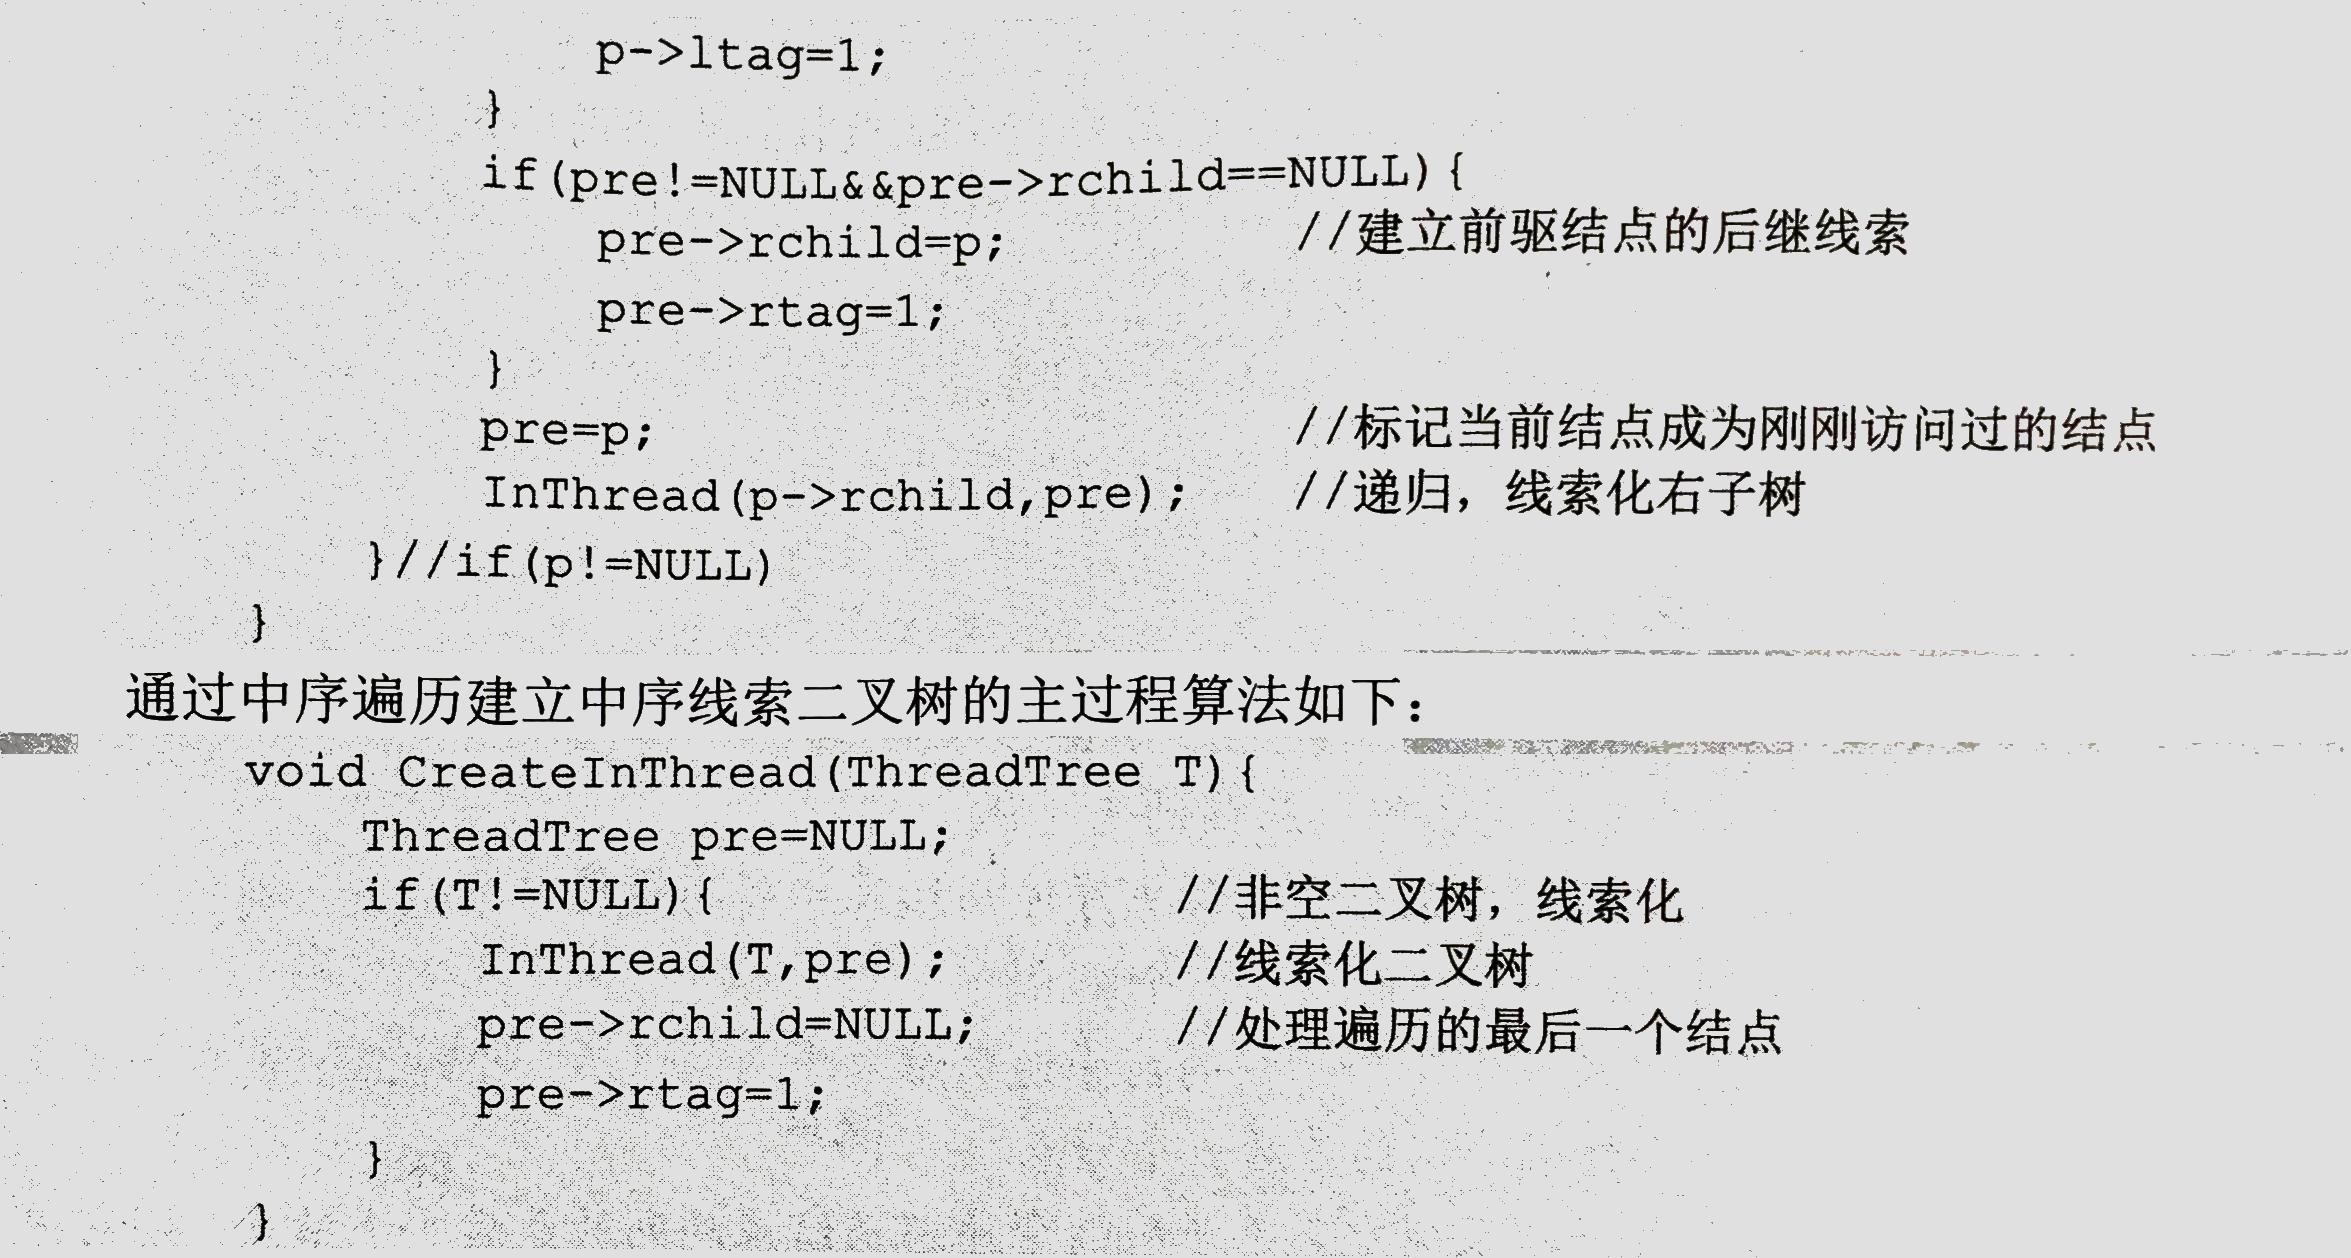
\includegraphics[scale=0.3]{example/chapter10/Img_181217112940976-1.jpg}
\end{figure}

\subsection{7.2}
\begin{lstlisting}[basicstyle=\small\ttfamily, caption={}, numbers=none]
算法思路:
构造无向网
\end{lstlisting}
\begin{lstlisting}[basicstyle=\small\ttfamily, caption={}, numbers=none]
Status CreateUND(MGraph &G) {
	//构造无向图
	scanf(&G.vexnum, &G.arcnum, &IncInfo);
	for (int i = 0; i < G.vexnum; ++i) {
		scanf(&G.vexs[i]);// 构造顶点向量
	}
	for (i = 0; i < G.vexnum; ++i) {// 初始化邻接矩阵
		for (j = 0; j < G.vexnum; ++j) {
			G.arcs[i][j] = { INFINITY, NULL };
		}
	}
	for (k = 0; k < G.vexnum; k++) {
		scanf(&v1, &v2, &w);
		i = LocateVex(G, v1); j = LocateVex(G, v2); // 确定v1和v2在G中的位置
		G.arcs[i][j].adj = w; // 弧的全职
		if (IncInfo) Input(*G.arcs[i][j].info);// 若弧含有相关信息则输入
		G.arcs[j][i] = G.arcs[i][j];
	}
	return OK;
}
\end{lstlisting}


\subsection{7.2}
\begin{lstlisting}[basicstyle=\small\ttfamily, caption={}, numbers=none]
算法思路:
采用十字链表存储表示,构造有向图G
\end{lstlisting}
\begin{lstlisting}[basicstyle=\small\ttfamily, caption={}, numbers=none]
			Status CreateDG(OLGraph &G) {
				scanf(&Gvexnum, &G.arcnum, &IncInfo);
				for (int i = 0; i < G.vexnum; ++i) {
					scanf(&G.xlist[i].data);// 输入顶点值
					G.xlist[i].firstin = NULL; G.xlist[i].firstout = NULL;
				}
				for (k = 0; k < G.arcnum; k++) {
					scanf(&v1, &v2);// 输入一条弧的起点和终点
					i = LocateVex(G, v1); j = LocateVex(G, v2);
					p = (ArcBox *)malloc(sizeof(ArcBox));
					*p = { i,j,G.xlist[j].firstin, G.xlist[i].firstout,NULL };
					//{tailvex, headvex, hlink, tlink, info}
					G.xlist[j].firstin = G.xlist[i].firstout = p;// 完成在入弧和出弧链头的插入
					if (IncInfo)Input(*p->info);
				}
			}

\end{lstlisting}


\subsection{7.5}
\begin{lstlisting}[basicstyle=\small\ttfamily, caption={}, numbers=none]
算法思路:
DFS
\end{lstlisting}
\begin{lstlisting}[basicstyle=\small\ttfamily, caption={}, numbers=none]
void DFS(Graph G, int v) {
	visited[v] = true;
	VisitFunc(v);
	for (w = FirstAdjVex(G, v); w >= 0; w = nextAdjVex(G, v, w)) {
		if (!visited[w])
			DFS(G, w);
	}
}
\end{lstlisting}


\subsection{7.6}
\begin{lstlisting}[basicstyle=\small\ttfamily, caption={}, numbers=none]
算法思路:
BFS
\end{lstlisting}
\begin{lstlisting}[basicstyle=\small\ttfamily, caption={}, numbers=none]
void BFSTraverse(Graph G, Status(*Visit)(int v)) {
	for (v = 0; v < G.vexnum; ++v) {
		visited[v] = FALSE;
	}
	InitQueue(Q);
	//初始化
	for (v = 0; v < G.vexnum; ++v) {
		if (!visited[v]) {
			visited[v] = true;
			Visit(v);
			EnQueue(Q, v);
			while (!QueueEmpty(Q)) {
				DeQueue(Q, u); // 对头元素出对,并置为u;
				for (w = FirstAdjVex(G, u); w >= 0; w = NextAdjVex(G, u, w)) {//w 为 u尚未访问的邻接顶点
					if (!Visit[w]) {
						Visited[w] = true;
						Visit(w);
						EnQueue(Q, W);
					}
				}
			}
		}
	}
}

\end{lstlisting}

\subsection{7.12}
\begin{lstlisting}[basicstyle=\small\ttfamily, caption={}, numbers=none]
算法思路:
拓扑排序
\end{lstlisting}
\begin{lstlisting}[basicstyle=\small\ttfamily, caption={}, numbers=none]
Status TopologicalSort(ALGraph G) {
	// 有向图采用邻接表存储结构
	// 若G 无回路,则输出G的顶点的一个拓扑序列并返回OK,否则ERROR
	FindInDegree(G, indegree);// 对各顶点求入读 indegree[0..vernum-1];
	InitStack(S);
	for (i = 0; i < G.vexnum; ++i) {
		if (!indegree[i]) Push(S, i);// 如果入度为0进栈
	}
	count = 0;
	while (!StackEmpty(S)) {
		Pop(S, i);
		printf(i, G.vertices[i].data); // 输出i号顶点并计数
		++count;
		for (p = G.vertices[i].firstarc; p; p = p->nextarc) {
			k = p->adjvex; // 对i 号顶点的每个邻接点的入读减1
			if (!(--indegree[k]))
				Push(S, k);// 若入度为0则入栈
		}
	}
	if (count < G.vexnum) return ERROR;// 该有向图有回路
	else
		return OK;
}

\end{lstlisting}

\subsection{9.1}
\begin{lstlisting}[basicstyle=\small\ttfamily, caption={}, numbers=none]
算法思路:
在数组里面查找某个元素
\end{lstlisting}
\begin{lstlisting}[basicstyle=\small\ttfamily, caption={}, numbers=none]
int Serach_Seq(SSTable ST, KeyType key) {
	// 在顺序表ST中顺序查找其关键字等于key的数据元素,若找到,则函数值为
	// 该元素在表中的位置,否则为0
	ST.elem[0].key = key;
	for (i = ST.length; !EQ(ST.elem[i].key, key); --i);
	return i;
}
\end{lstlisting}

\subsection{9.1}
\begin{lstlisting}[basicstyle=\small\ttfamily, caption={}, numbers=none]
算法思路:
折半查找
\end{lstlisting}
\begin{lstlisting}[basicstyle=\small\ttfamily, caption={}, numbers=none]
int Search_Bin(SSTable ST, KeyType key) {
	// 在有序表ST中折半查找其关键字等于key的数据元素。若找到,则函数值为
	// 该元素在表中的位置,否则为0
	low = l; high = ST.length;
	while (low <= high) {
		mid = (low + high) / 2;
		if (EQ(key, ST.elem[mid].key)) return mid;
		else if (LT(key, ST.elem[mid].key)) high = mid - 1;
		else
			low = mid + 1;
	}
	return 0;
}
\end{lstlisting}

\subsection{10.1}
\begin{lstlisting}[basicstyle=\small\ttfamily, caption={}, numbers=none]
算法思路:
直接插入排序
\end{lstlisting}
\begin{lstlisting}[basicstyle=\small\ttfamily, caption={}, numbers=none]
void InsertSort(SqList &L) {
	// 对顺序表L作直接插入排序
	for (i = 2; i <= L.length; ++i) {
		if (LT(L.r[i].key, L.r[i - 1].key)) {
			L.r[0] = L.r[i]; // 哨兵
			L.r[i] = L.r[i - 1];
			for (j = i - 2; LT(L.r[0], L.r[j].key); --j) {
				L.r[j + 1] = L.r[j]; // 记录后移
			}
			L.r[j + 1] = L.r[0];//插入到正确位置
		}
	}
}
\end{lstlisting}

\subsection{10.2}
\begin{lstlisting}[basicstyle=\small\ttfamily, caption={}, numbers=none]
算法思路:
折半插入排序
\end{lstlisting}
\begin{lstlisting}[basicstyle=\small\ttfamily, caption={}, numbers=none]
void BInsrtSort(SqList &L) {
	for (i = 2; i <= L.length; i++) {
		L.r[0] = L.r[i];
		low = 1; high = i - 1;
		while (low <= high) {
			m = (low + high) / 2;
			if (LT(L.r[0].key, L.r[m].key)) high = m - 1;
			else low = m + 1;
		}
		for (j = i - 1; j >= high + 1; --j) {
			L.r[j + 1] = L.r[j];//记录后移
		}
		L.r[hgih + 1] = L.r[0];
	}
}
\end{lstlisting}


\subsection{10.5}
\begin{lstlisting}[basicstyle=\small\ttfamily, caption={}, numbers=none]
算法思路:
希尔排序
\end{lstlisting}
\begin{lstlisting}[basicstyle=\small\ttfamily, caption={}, numbers=none]
void ShellInsert(SqList &L, int dk) {
	// 对顺序表L做一趟希尔排序。本算法时和一趟直接插入排序相比做了以下修改
	// 1.前后记录位置的增量时dk,而不是1
	// 2.r[0]只是暂存单元不是哨兵。当j<=0时,插入位置已找到。
	for (i = dk + 1; i <= L.length; i++) {
		if (LT(L.r[i].key, L.r[i - dk].key)) {
			L.r[0] = L.r[i];
			for (j = i - dk; j > -&&LT(L.r[0].key, L.r[j].key); j -= dk) {
				L.r[j + dk] = L.r[j];
			}
			L.r[j + dk] = L.r[0];
		}
	}
}
void ShellShort(SqList &L, int dlta[], int t) {
	for (k = 0; k < t; ++k) {
		ShellInsert(L, dlta[k]);
	}
}
\end{lstlisting}


\subsection{10.6}
\begin{lstlisting}[basicstyle=\small\ttfamily, caption={}, numbers=none]
算法思路:
快速排序
\end{lstlisting}
\begin{lstlisting}[basicstyle=\small\ttfamily, caption={}, numbers=none]
int Partition(SqList &L, int low, int high) {
	// 交换顺序表L中字表L.r[low...high]的记录,使枢轴记录到位,并返回其所在位置,此时
	// 在它之前(后)的记录均不大(小)于它。
	pivotkey = L.r[low].key;// 用子表的第一个记录做枢轴量技术
	while (low < high) {
		while (low < high && L.r[high].key >= pivotkey) --high;
		swap(L.r[low], L.[high]);
		while (low < high && L.r[low].key <= pivotkey) ++low;
		swap(L.r[low], L.r[high]);
	}
	return low;
}
void QSort(SqList &L, int low, int high) {
	if (low < high) {
		povotloc = Partition(L, low, high);
		Qsort(L, low, pivotloc - 1);
		QSort(L, pivotloc + 1, high);
	}
}
\end{lstlisting}


\subsection{10.6}
\begin{lstlisting}[basicstyle=\small\ttfamily, caption={}, numbers=none]
算法思路:
堆排序
\end{lstlisting}
\begin{lstlisting}[basicstyle=\small\ttfamily, caption={}, numbers=none]
void AdjustDown(int A[],int k, int len) {
	A[0] = A[k];
	for (i = 2 * k; i <= len; i*=2) {
		if (i < len&&A[i] < A[i + 1]) {
			i++;
		}
		if (A[0] >= A[i]) break;
		else {
			A[k] = A[i];
			k = i;
		}
	}
	A[k] = A[0];
}

void BuildMaxHeap(int A[], int n) {
	for (int i = n / 2; i > 0; i--) {
		AdjustDown(A, len, i);
	}
}
void HeapSort() {
	BuildMaxHeap(A, len);
	for (i = len; i > 1; i--) {
		swap(A[i], A[1]);
		AdjustDown(A, 1, i - 1);
	}
}
\end{lstlisting}






